\documentclass[12pt, a4paper, UTF8, fontset=windows]{ctexbook}
\usepackage{amsmath, amsthm, amssymb, amsfonts, bm, color, fancyhdr, framed, geometry, graphicx, hyperref, lastpage, listings, mathrsfs, xcolor}


\linespread{1.5}
\definecolor{shadecolor}{RGB}{241, 241, 255}
\newcounter{problemname}
\newenvironment{problem}{\begin{shaded}\stepcounter{problemname}\par\noindent\textbf{Q\arabic{problemname}.}}{\end{shaded}\par}
\newenvironment{solution}{\par\noindent\textbf{Ans.}}{\par}

\geometry{left=20mm,right=20mm, top=20mm, bottom=22mm} % 页边距
\setlength{\headheight}{15pt}
\pagestyle{fancy} % 设置页脚页眉
\rhead{Assignment3} % 页眉右边
% \noindent % 取消首段缩进

\definecolor{mygreen}{rgb}{0,0.6,0}
\definecolor{mygray}{rgb}{0.5,0.5,0.5}
\definecolor{mymauve}{rgb}{0.58,0,0.82}
% 代码设置
\lstset{ 
backgroundcolor=\color{white},      % choose the background color
basicstyle=\footnotesize\ttfamily,  % size of fonts used for the code
columns=fullflexible,
tabsize=4,
breaklines=true,               % automatic line breaking only at whitespace
captionpos=b,                  % sets the caption-position to bottom
commentstyle=\color{mygreen},  % comment style
keywordstyle=\color{blue},     % keyword style
stringstyle=\color{mymauve}\ttfamily,  % string literal style
frame=single,
rulesepcolor=\color{red!20!green!20!blue!20},
language=c++,
xleftmargin=3em,
xrightmargin=3em
}


\begin{document}

\cfoot{\thepage\ / \pageref{LastPage}} % 页眉中间位添加内容:页码/总页码

\thispagestyle{empty}

\begin{figure}[t]
    \centering
    
\includegraphics[width=6cm]{../../src/images/logo.jpg}
\end{figure}

\vspace*{\fill}
    \begin{center}
        \Huge\textbf{Assignment3}
    \end{center}
\vspace*{\fill}

\begin{table}[b]
    \centering
    \large
    \begin{tabular}{ll}
    \textbf{课程:} & 算法设计与分析 \\
    \textbf{姓名:} & 雷翔 \\
    \textbf{学号:} & 2053932 \\
    \textbf{时间:} & 2023年5月 \\
    \end{tabular}
\end{table}


\newpage

\setcounter{page}{1} % 页码从当前页开始

\begin{problem}
    请用回溯法对下图求哈密顿回路问题(从 a 点开始),请详细给出解空间树,搜索过程及结果。
\end{problem}

\begin{solution}
    \begin{figure}[h]
        \centering
        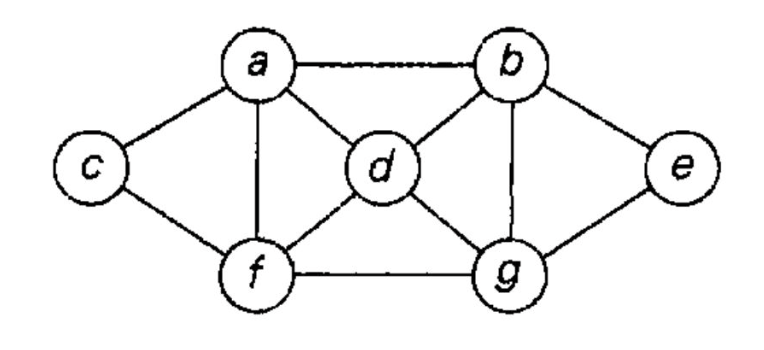
\includegraphics[width=8cm]{../../src/images/hw3-Q1.png}
    \end{figure}


    \vspace{2mm}  % 指定高度,添加空行

    1. 定义解空间
    
    X = \{abcdefga, abcdegfa, ···, agfedcba\}

    2. 解空间树
    \begin{figure}[h]
        \centering
        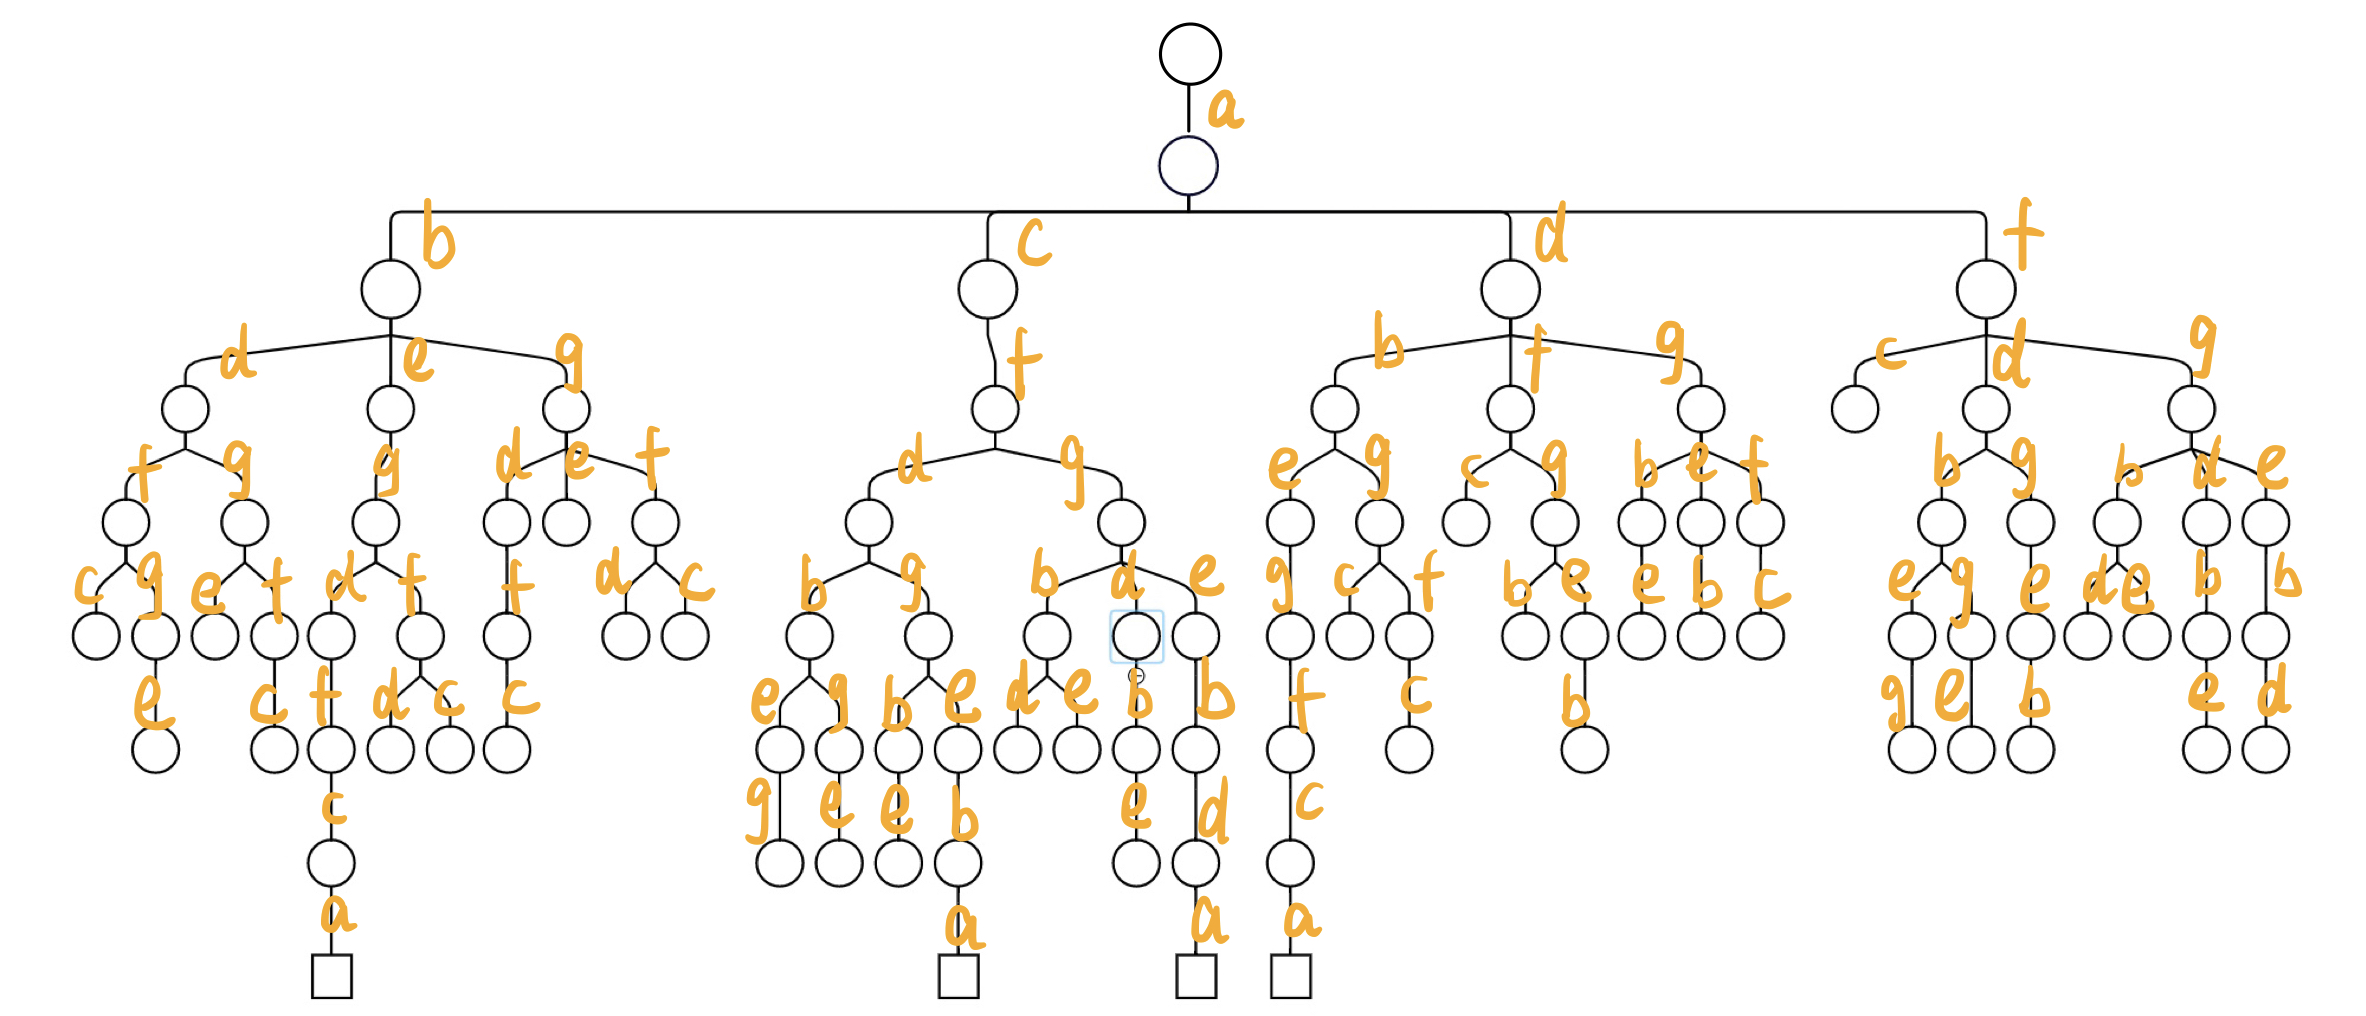
\includegraphics[width=15cm]{../../src/images/hw3-Q1-tree.jpg}
    \end{figure}

    3. 从 a 出发按 DFS 搜索整棵树

    a -> b -> d -> f -> c

    回溯到 f

    f -> g -> e

    回溯到 d

    d -> g -> e

    回溯到 g

    g -> f -> c

    回溯到 b


    b- > e -> g -> d -> f - > c -> a 得到第一个解

    其余解同理可得
    
    
\end{solution}

\newpage

\begin{problem}
    找零问题:给予币值为 1,3,5 的硬币若干(每种硬币个数无限多),如何用这些硬币组合,使得面额为 9,且硬币的的个数最少?请利用动态规划算法求其所有解。请给出算法伪代码并参考教材详细描 述算法的运行过程。
\end{problem}

\begin{solution}
    面值为 6 的组合的硬币最小个数可以由面值为 5、3、2 的组合的硬币最小个数中的最小值加 1 计算。

    记面额为 j 的硬币组合个数为 dp[j]
    
    初始条件:dp[0] = 0

    状态方程:
    \begin{equation}
        f(x)=
        \begin{cases}
        min \{dp[j-1]\} + 1                     & \text{1 <= j < 3}  \\
        min \{dp[j-1], dp[j-3]\} + 1            & \text{3 <= j < 5}  \\
        min \{dp[j-1], dp[j-3], dp[j-5]\} + 1   & \text{j >= 5}
        \end{cases}
    \end{equation}
    
    \begin{table}[htbp]
        \centering  % 显示位置为中间
        \caption{面额与最小硬币个数的对应关系}  % 表格标题
        \label{table1}  % 用于索引表格的标签
        %字母的个数对应列数,|代表分割线
        % l代表左对齐,c代表居中,r代表右对齐
        \begin{tabular}{|c|c|c|c|c|c|c|c|c|c|c|}  
            \hline  % 表格的横线
            j&0&1&2&3&4&5&6&7&8&9 \\  % 表格中的内容,用&分开,\\表示下一行
            \hline 
            dp[j]&0&1&2&1&2&1&2&3&2&3 \\
            \hline
        \end{tabular}
    \end{table}

    dp[1] = dp[0] + 1 = 1     
    
    dp[2] = dp[1] + 1 = 2     
    
    dp[3] = min\{dp[2], dp[0]\} + 1 = 1
    
    dp[4] = min\{dp[3], dp[1]\} + 1 = 2

    依次类推,dp[9] = min \{dp[8], dp[6], dp[4]\} + 1 = 3

    组合: 3 个币值为 3 元的硬币或 1 个币值为 1元 + 1 个币值为 3 元 + 1 个币值为 5 元

    伪代码:

    \begin{lstlisting}
    // 求面额为 n 的硬币最小个数
    function dp(n) {
        for i <- 0 to n  // 得到一个大小为 n + 1,值为 0 的数组
            do dp[i] <- 0
        for j <- 1 to n do
            if j >= 1 && j < 3
                dp[j] = dp[j-1] + 1
            else if j >= 3 && j < 5
                dp[j] = min(dp[j-1], dp[j-3]) + 1
            else 
                dp[j] = min(dp[j-1], dp[j-3], dp[j-5]) + 1

        return dp  // 返回结果数组
    }
    \end{lstlisting}
\end{solution}


\begin{problem}
    请用分支限界法对背包问题的以下示例求解,请详细给出解空 间树,搜索过程及结果。
\end{problem}
    

\begin{solution}
    \begin{figure}[h]
        \centering
        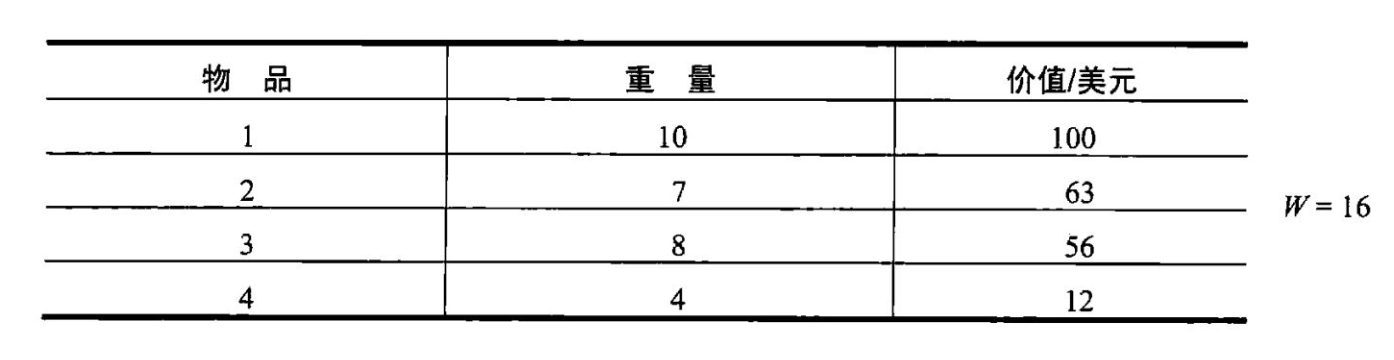
\includegraphics[width=12cm]{../../src/images/hw3-Q3.png}
    \end{figure}
    
    1. 定义解空间

    X = \{(0, 0, 0, 0), (0, 0, 0, 1), ···, (1, 1, 1, 1)\}

    2. 定义解空间树

    \begin{figure}[h]
        \centering
        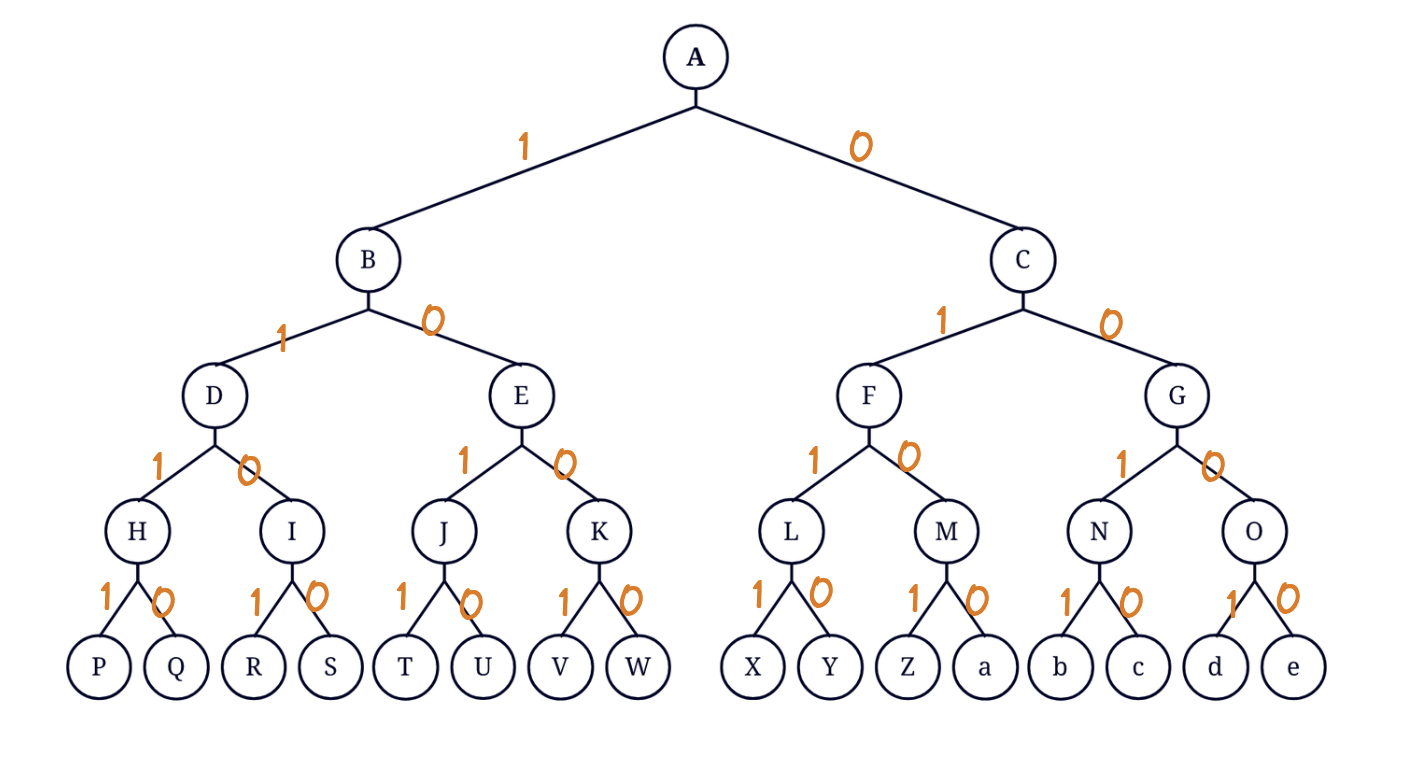
\includegraphics[width=15cm]{../../src/images/hw3-Q3-tree.png}
    \end{figure}


    3. 按 BFS 方式进行搜索,采用优先队列 

    优先级取决于背包中已经装袋的物品价值加上剩下的最大价值物品装满袋的价值总和

    w:袋子里的重量

    v:袋子里物品的价值

    UB:上界

    \newpage

    搜索过程:
    
    \begin{figure}[htb]
        \centering
        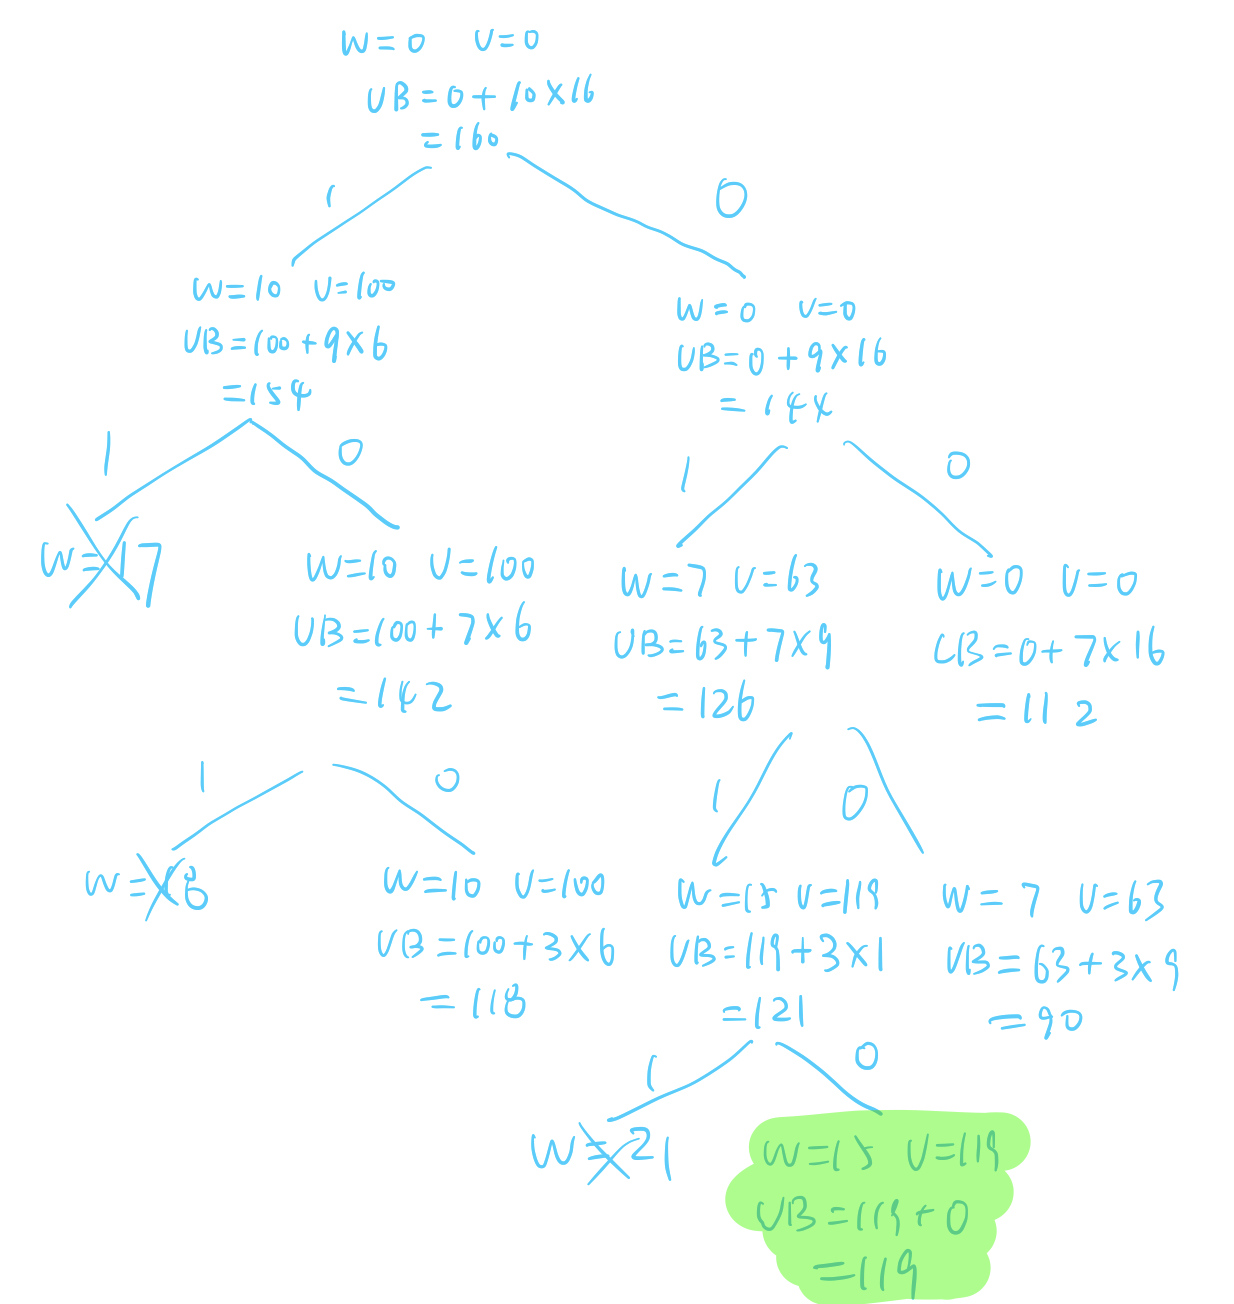
\includegraphics[width=15cm]{../../src/images/hw3-Q3-solution.jpg}
    \end{figure}

    结果:选择物品 2 和物品 3,最大价值为 119
\end{solution}

\newpage 

\begin{problem}
    对于图 3,应用分支限界法求解从 a 点开始的 TSP 问题,请详细给出解空间树,搜索过程及最优解。
\end{problem}


\begin{solution}
    \begin{figure}[htb]
        \centering
        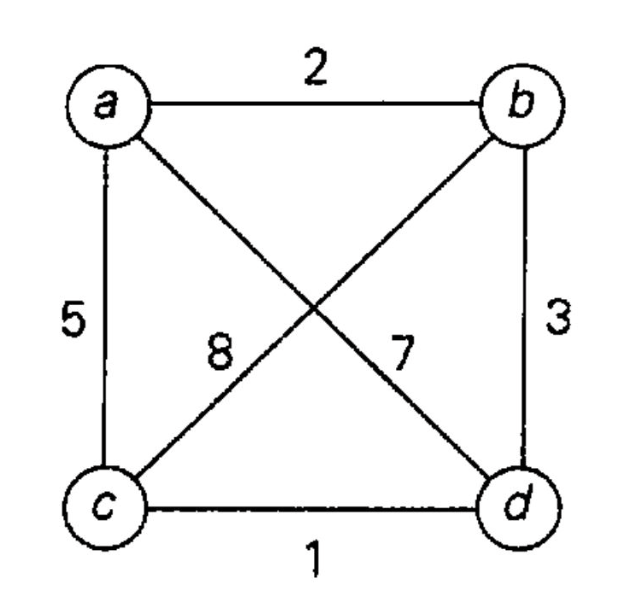
\includegraphics[width=6cm]{../../src/images/hw3-Q4.png}
    \end{figure}

    1. 定义解空间

    X = \{abcda, abdca, acbda, acdba, adbca, adcba\}

    2. 构造解空间树

    \begin{figure}[h]
        \centering
        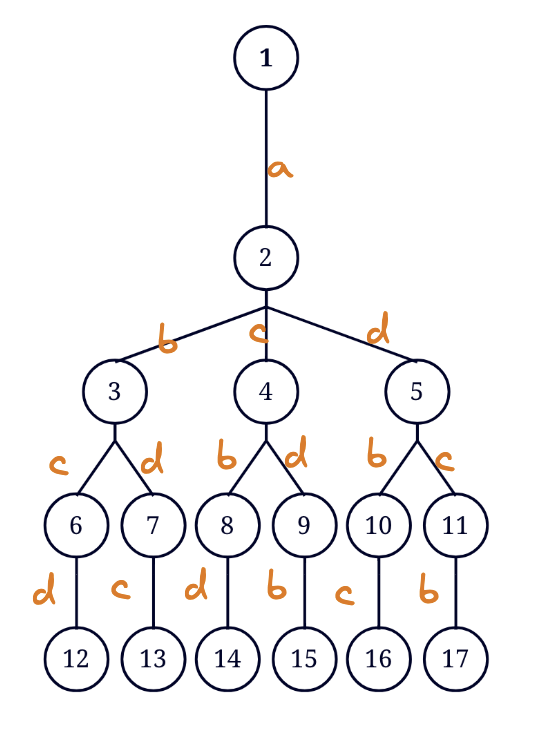
\includegraphics[width=8cm]{../../src/images/hw3-Q4-tree.png}
    \end{figure}

    \newpage

    3. 按 BFS 方式进行搜索,采用优先队列 

    搜索过程:
    
    \begin{figure}[h]
        \centering
        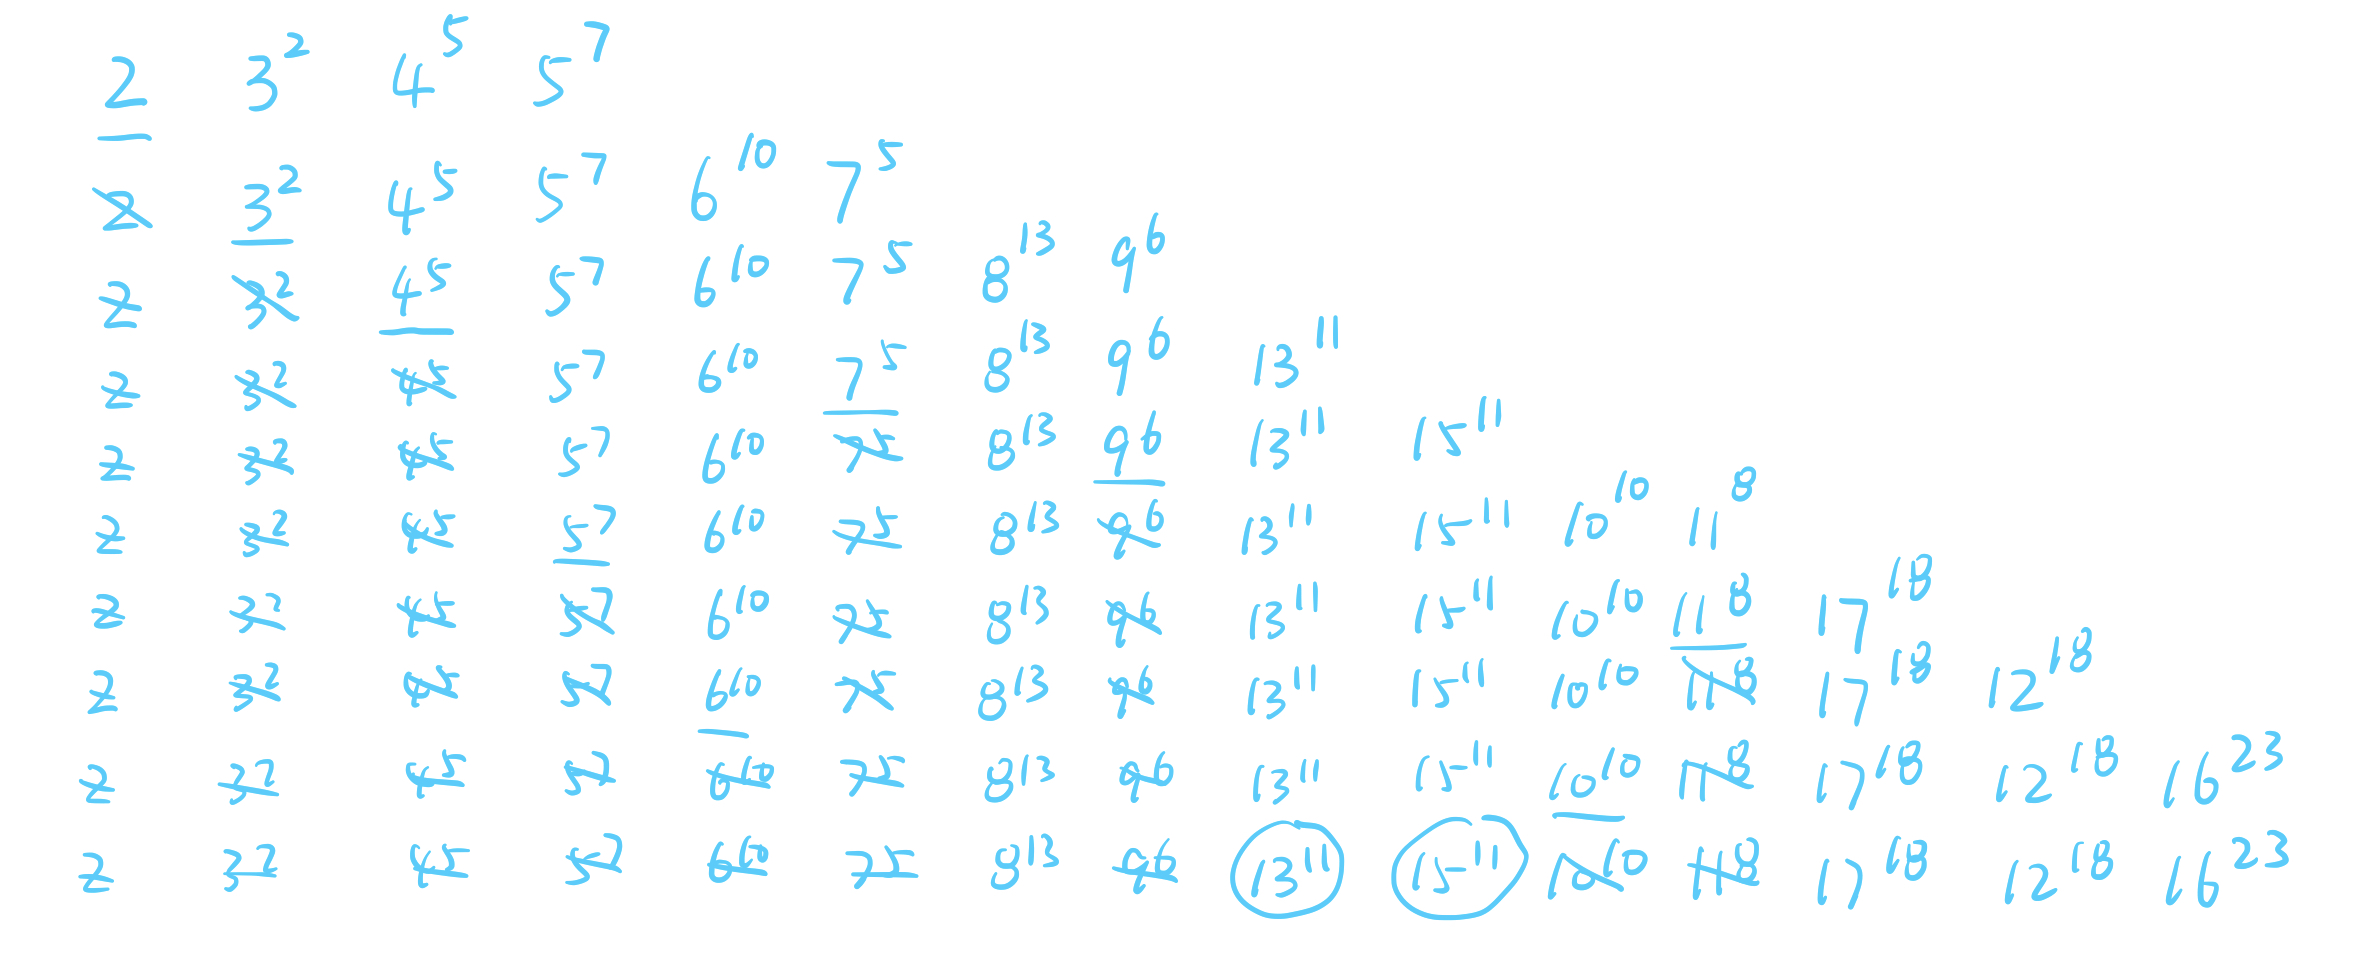
\includegraphics[width=15cm]{../../src/images/hw3-Q4-solution.jpg}
    \end{figure}

    结果:a -> b -> d -> c -> a 和 a -> c -> d -> b -> a

    最短路径为 11 
\end{solution}

\begin{problem}
    在一个类似谜题的游戏中,等边三角形的板上布置了 15 个孔。 在初始的时候,如下图所示,除了一个孔,所有孔都插上了插棒。一 个插棒可以跳过它的直接邻居,移到一个空白的位置上。这一跳会把 被跳过的邻居从板上移走。

    请使用回溯算法,描述求解该谜题的下列版本的主要思路并给出算法的伪代码:

    a 已知空孔的位置,求出消去 13 个棒的最短步骤,对剩下的插棒的最终位置不限。

    b 已知空孔的位置,求出消去 13 个棒的最短步骤,剩下的插棒最终要落在最初的空孔上。
\end{problem}

\begin{solution}
    \begin{figure}[h]
        \centering
        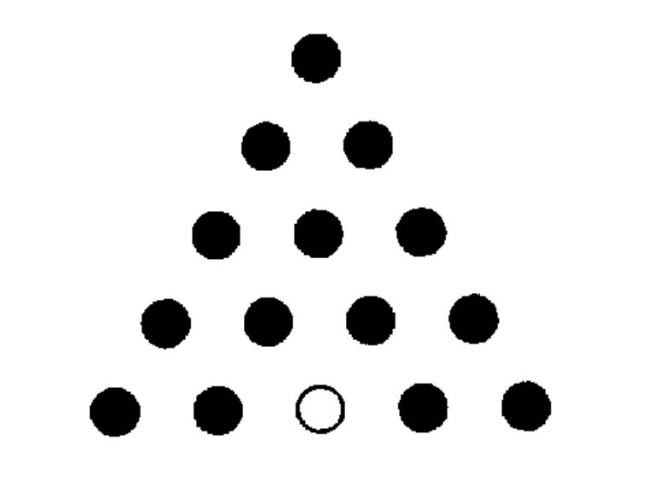
\includegraphics[width=8cm]{../../src/images/hw3-Q5.png}
    \end{figure}

    \newpage 

    % \begin{figure}[h]
    %     \centering
    %     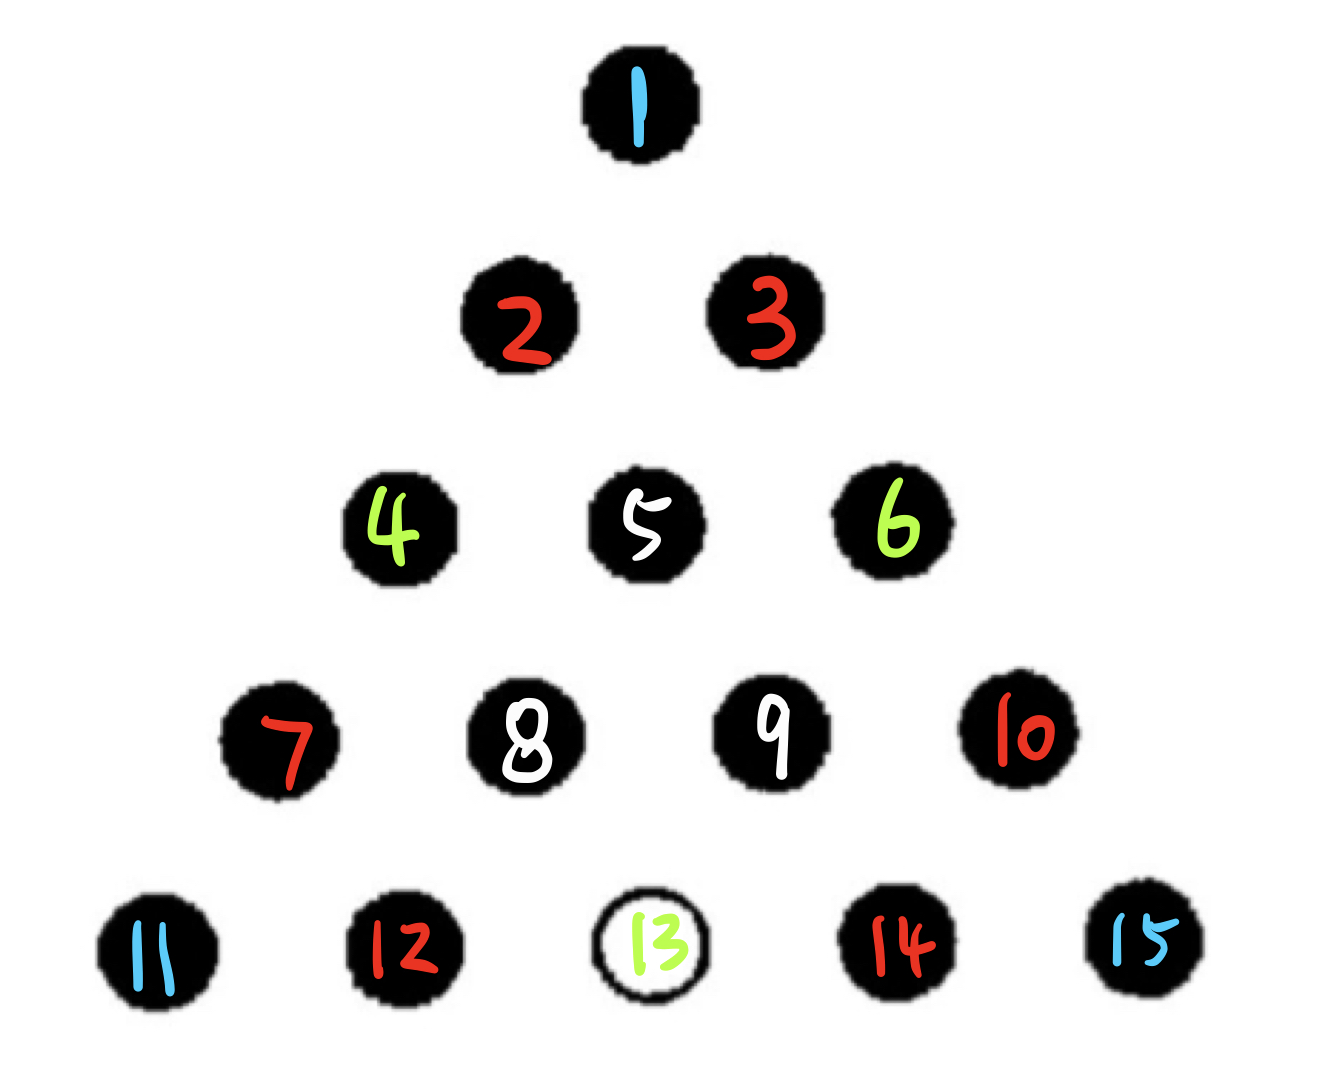
\includegraphics[width=8cm]{../../src/images/hw3-Q5-solution.jpg}
    % \end{figure}

    % 由于等边三角形的特殊形状,以上颜色相同的数字对应的孔是等效的,要么都无解,要么都有相同的解。

    a.

    首先初始化状态,主要包括定义棋盘数组,表示棋盘状态,用 1 表示有插棒,0 表示空孔,记录当前空孔位置的变量以及一个记录最短步数的变量。

    从当前空孔位置开始,依次向四周能跳跃的方向跳跃,并将路径上的插棒移除。如果已经消去了 13 个插棒,就更新最短步数变量,如果当前步数超过最短步数变量,就回溯到上一步。

    \begin{lstlisting}
    // 从 from 跳到 to,中间经过 in
    // empty_hole 表示当前空孔的位置
    function backtrack(board, empty_hole, removed_count, step) {
        if removed_count == 13 {  // 消除 13 个棒
            if step < min_step {
                min_step = step
            }
            return
        }
        for each in 临近的插棒 {
            如果将跳跃到的位置是空孔empty_hole {  // 对应 to 位置
                将跳过的插棒移除 // 对应 in 位置
                backtrack(board, 跳过的位置in, removed_count + 1, step + 1)
                恢复跳过的插棒in // 对应 in 位置
            }
        }
    }
    \end{lstlisting}

    b. 

    在 a 的基础上,保留下最初的空孔位置。在消除 13 个棒后,判断当前空孔位置是否为最初的空孔位置,如果是,就更新最短步数变量,否则回溯到上一步。

    \begin{lstlisting}
    // 从 from 跳到 to,中间经过 in
    // empty_hole 表示当前空孔的位置
    // target_hole 表示最终要落在的空孔的位置
    function backtrack(board, empty_hole, removed_count, step) {
        if removed_count == 13 and empty_hole == target_hole {  // 消除 13 个棒,且剩下的插棒落在最初的空孔
            if step < min_step {
                min_step = step
            }
            return
        }
        for each in 临近的插棒 {
            如果将跳跃到的位置是空孔empty_hole {  // 对应 to 位置
                将跳过的插棒移除 // 对应 in 位置
                backtrack(board, 跳过的位置in, removed_count + 1, step + 1)
                恢复跳过的插棒in // 对应 in 位置
            }
        }
    }
    \end{lstlisting}

\end{solution}

\end{document}